\section{Oefeningen}
\begin{oef}
De rechte $r$ gaat door punten $A$ en $B$. Stel het functievoorschrift op voor $r$. Zoek het nulpunt en het snijpunt met de verticale as.
\begin{enumerate}
\item $A(2,5)$ en $B(4,-1)$
\item $A(-2,-4)$ en $B(3,-4)$
\item $A(3,-1)$ en $B(3,6)$ 
\end{enumerate}
     \begin{opl}
\begin{enumerate}
\item $f(x)=-3x+11$, nulpunt $(\frac{11}{3}, 0)$ en snijpunt met de $y$-as: $(0,11)$
\item $f(x)=-4$, dus een constante functie. Deze functie heeft geen nulpunt en het snijpunt met de $y$-as is $(0,-4)$.
\item Deze rechte heeft als vergelijking $x=3$. Het is een verticale rechte en dus geen functie. Het heeft dan ook geen zin om te spreken over nulpunt en snijpunt met de $y$-as.
\end{enumerate}
     \end{opl}
\end{oef}

\begin{oef}
Figuur~\ref{fig:rechtenoef2} toont enkele rechten in een assenkruis. Stel een vergelijking op van de rechten. Welke stellen functies voor?
\begin{figure}[htbp]
    \centering
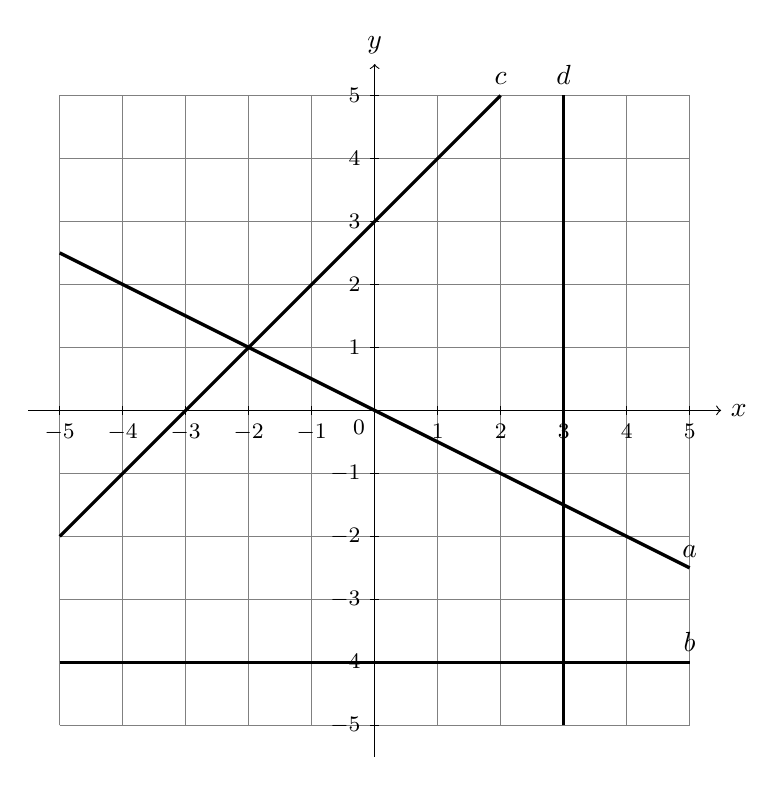
\begin{tikzpicture}[scale=0.8]
\draw[help lines] (-5,-5) grid  (5,5);
\draw[->] (-5.5,0) -- (5.5,0) node[right] {$x$};
\draw[->] (0,-5.5) -- (0,5.5) node[above] {$y$};
\foreach \x in {-5,...,-1,1,2,...,5}
	\draw[shift={(\x,0)}] (0pt,2pt) -- (0pt,-2pt) node[below] {\footnotesize $\x$};
\foreach \y in {-5,...,-1,1,2,...,5}
	\draw[shift={(0,\y)},color=black] (2pt,0pt) -- (-2pt,0pt) node[left] {\footnotesize $\y$};
\node [below left] at (0,0) {\footnotesize 0};
\draw[very thick] (-5,2.5) -- (5,-2.5) node[above] {$a$};
\draw[very thick] (-5,-4) -- (5,-4) node[above] {$b$};
\draw[very thick] (-5,-2) -- (2,5) node[above] {$c$};
\draw[very thick] (3,-5) -- (3,5) node[above] {$d$};
\end{tikzpicture}
\caption{Zoek een vergelijking voor deze rechten}
    \label{fig:rechtenoef2}
\end{figure}
\begin{opl} Enkel rechte $d$ is geen functie \\
$a\leftrightarrow y=-\frac{1}{2}x$\\
$b \leftrightarrow y=-4 $\\
$c \leftrightarrow y=x+3$\\
$d \leftrightarrow x=3$
\end{opl}
\end{oef}


\begin{oef}
Je twijfelt tussen drie verschillende tariefplannen voor telefonie. Je bent enkel geïnteresseerd in bellen (dus niet in SMS of data). Bij Proximus stelt men je het tarief `free call' voor. Echt `free' is het wel niet: je betaalt \euros{30} per maand, maar je mag wel onbeperkt bellen naar alle netwerken. Mobistar vertelt je dat hun tarief `olifant' het goedkoopste is. Je betaalt een abonnementskost van \euros{15}. Je mag dan wel een uur gratis bellen. Als je gratis uur opgebruikt is, worden je telefoongesprekken betalend tegen \euros{0,25} per minuut. Base beweert dat je nergens goedkoper belt dan met hun `simpel' herlaadkaart: geen abonnementskosten, enkel \euros{0,40} per belminuut.

Maak een figuur van de verschillende tarieven (kostprijs i.f.v. de beltijd). Duid op de figuur aan wat de goedkoopste formule is voor elke beltijd. Geef een overzichtelijk antwoord.

Stel dat je telkens voor de goedkoopste formule gaat. Hoeveel kosten dan respectievelijk 10, 100 en 1000 belminuten?
\begin{opl}
Tot een maandelijkse beltijd van 37,5 minuten is Base het goedkoopst. Tussen 37,5 en 120 minuten kan je best Mobistarklant worden. Voor wie meer belt dan twee uur per maand is Proximus het goedkoopst. 
Voor 10 belminuten kies je dus Base met een kostprijs van $10\cdot 0,40=4$ euro. Als je 100 minuten per maand belt, ben je goedkoopst bij Mobistar. Dat kost je dan \euros{25}. Wie 1000 minuten belt, hoeft niet te twijfelen: kies Proximus en dus kost het je \euros{30}.
\end{opl}
\end{oef}

\begin{oef}
De snelste supercomputer (figuur~\ref{fig:ibmBG}) in 2012 is de IBM Blue Gene Sequoia\footnote{\url{http://www.top500.org/list/2012/06/100}}.  Deze computer haalt 16324 TFlops (Teraflops). 
\begin{figure}[hbtp]
\centering
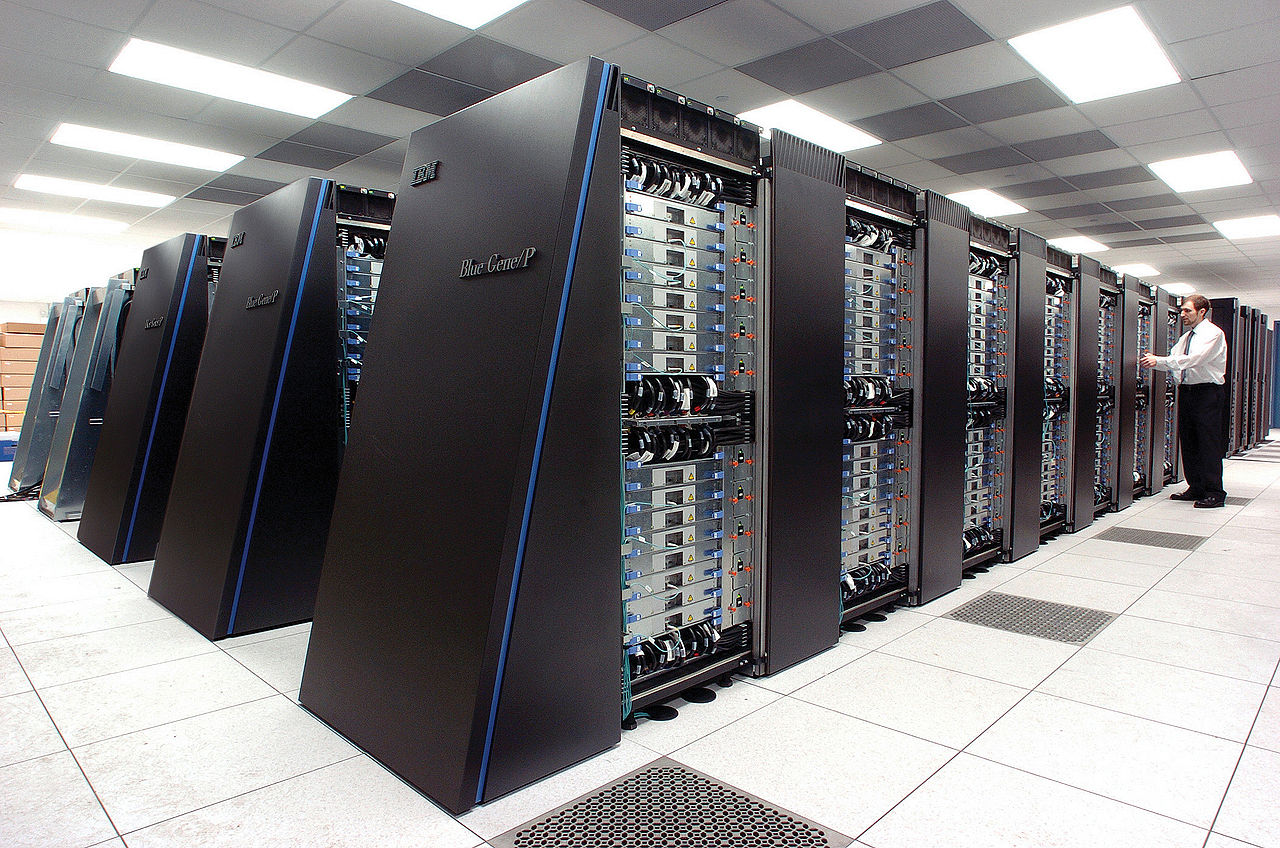
\includegraphics[width=\textwidth]{figuren/eerstegraadsfuncties/IBMBlueGene.jpg}
\caption{IBM Blue Gene supercomputer}
\label{fig:ibmBG}
\end{figure}

Eén teraflop is $10^{12}$ floating point berekeningen per seconde. Het vermogen bedraagt \SI{7,890}{\mega\watt}. Ter vergelijking: de grootste kerncentrale in Doel (4) heeft een vermogen van ongeveer \SI{1000}{\mega\watt}, wat betekent dat ongeveer 126 van dergelijke supercomputers heel de elektrische productie van Doel 4 zouden opgebruiken. Stel dat het verband tussen rekensnelheid (in TFlops) en vermogen (in \si{\mega\watt}) rechtevenredig is, wat zou dan het vermogen worden als er over afzienbare  tijd een supercomputer \num{100000} TFlops haalt (dat zijn dus \num{100000000000000000} floating point berekeningen per seconde)? Is de veronderstelling dat dit verband rechtevenredig is te verdedigen, denk je?
\begin{opl}
Eerst en vooral: de aanname van rechtevenredigheid is niet te verdedigen. Als je naar de geciteerde URL in de opgave gaat kijken, merk je dat men niet anders kan dan ook het verbruik (koeling, \ldots) in aanmerking nemen en proberen dit zo laag mogelijk te houden. Als we dan toch de evenredigheid volgen, bekomen we het antwoord dat getoond wordt in figuur~\ref{fig:rekensnelheidvermogen}.
\begin{figure}[htbp]
    \centering
\begin{tikzpicture}[x=0.08cm,y=0.15cm]
%\draw[help lines] (-5,-5) grid  (5,5);
\draw[->] (-2,0) -- (105,0) node[right] {1000 TFlops};
\draw[->] (0,-1) -- (0,52) node[above] {\si{\mega\watt}};
\foreach \x in {10,20,...,100}
	\draw[shift={(\x,0)}] (0pt,2pt) -- (0pt,-2pt) node[below] {\footnotesize $\x$};
\foreach \y in {10,20,...,50}
	\draw[shift={(0,\y)},color=black] (2pt,0pt) -- (-2pt,0pt) node[left] {\footnotesize $\y$};
\node [below left] at (0,0) {\footnotesize 0};
\draw[thick] (0,0) -- (110,53.17);
\draw[dashed] (16.324,0) |- (0,7.89);
\filldraw [red] (16.324,7.89) circle (2pt) node[below right] {$(16,324;7,89)$};
\draw[dashed] (100,0) |- (0,48.33);
\filldraw [red] (100,48.33) circle (2pt) node[below right] {$(100;48,33)$};
\end{tikzpicture}
\caption{Verband tussen vermogen en rekensnelheid}
    \label{fig:rekensnelheidvermogen}
\end{figure}
\end{opl}
\end{oef}

\begin{oef}
Een harde schijf van 500 GB kost \euros{60}. Die van 2 TB kost \euros{130}. Bij gebrek aan andere informatie gaan we ervan uit dat het verband tussen opslagcapaciteit en prijs lineair is. Hoeveel zou volgens dit verband dan een harde schijf van 1,5 TB kosten? Je mag voor de eenvoud een TB gelijk stellen aan 1000 GB (wat is de juiste waarde?). Deze techniek noemen we `lineaire interpolatie'. Wat denk je in dit verband over de prijs van een harde schijf van 5 TB?
\begin{opl}
Stel de vergelijking van de rechte door de punten $(500,60)$ en $(2000,130)$. Vul dan in deze vergelijking $x=1500$ in en je bekomt \euros{106,67}. Bij 5 TB spreken we over extrapolatie en dat is meestal vrij gevaarlijk. Hoe meer data op een harde schijf, des te groter wordt de technische uitdaging en des te kleiner worden componenten, sporen enz. Een lineair verband zal dan zeker geen goede benadering zijn!
\end{opl}
\end{oef}

\begin{oef}
In Heverlee gelden volgende tarieven voor drinkwater (exclusief 6\% BTW):
\begin{itemize}
\item Vaste vergoeding: 47 \euro/jaar 
\item Verbruik van het drinkwater:  \SI{2}{\euro\per\cubic\metre} 
\item Bijdrage voor de zuivering van drinkwater: \SI{0,9}{\euro\per\cubic\metre}  
\item Bijdrage voor de afvoer van drinkwater: \SI{1,3}{\euro\per\cubic\metre}  
\end{itemize}
\begin{enumerate}
\item Bepaal het verband tussen het te betalen bedrag aan de drinkwatermaatschappij en de verbruikte hoeveelheid water
\item Een Vlaming verbruikt gemiddeld \SI{45}{\cubic\metre}   water per jaar. Van de overheid krijgt hij \SI{15}{\cubic\metre} gratis, maar hij moet wel de bijdrage voor de zuivering en afvoer betalen. Hoe groot is de gemiddelde factuur van de Vlaming?
\end{enumerate}

\begin{opl}
\begin{enumerate}
\item Veranderlijken benoemen: $x$ is verbruikte hoeveelheid drinkwater; $B$ is het te betalen bedrag
\item $B(x)=47+(2+0,9+1,3)\cdot x=47+4,2x$
\item $B_2(x)=47+2\cdot (x-15)+(0,9+1,3)\cdot x=17+4,2\cdot x$ \\
$B_2(45)=206$. De gemiddelde Vlaming betaalt \euros{206} per jaar.
\end{enumerate}
\end{opl}
\end{oef}

\begin{oef}
In	Vlaanderen	bestaat 	je	drinkwaterfactuur	steeds	uit	twee	delen:	het	verbruik	(\SI{2}{\euro\per\cubic\metre})  	en een	bijdrage	voor	zuivering	en	afvoer	(\SI{2.2}{\euro\per\cubic\metre}).		Voor	 de	 eerste	\SI{15}{\cubic\metre} hoef	je	
niet	te	betalen	  voor	het	verbruik.	Je	moet	dan	enkel	betalen	 voor	zuivering	en	 afvoer.	

In	 Brussel	geldt	een	getrapte	tarifering: 	naargelang	je	meer	verbruikt,	 wordt	de	 prijs	per	
\SI{}{\cubic\metre} duurder.	Voor	schijf 1	(0--15 \SI{}{\cubic\metre})	betaal	je	\SI{1,88}{\euro\per\cubic\metre}.	Voor	schijf	2	(15--30 \SI{}{\cubic\metre})	
betaal	je	\SI{3,38}{\euro\per\cubic\metre}.	Voor	schijf	3	(30-60 \SI{}{\cubic\metre})	betaal	je	\SI{4}{\euro\per\cubic\metre}.	
Voor	het	water	meer dan	\SI{60}{\cubic\metre} betaal	je	zelfs	 \SI{7,33}{\euro\per\cubic\metre}.
\begin{enumerate}
\item  Definieer	in	Scilab	de	 functies	“vlaanderen” 	en	 “brussel”	die	het	te	betalen	 bedrag	
in	Vlaanderen	resp.	\ Brussel	berekent	in	functie	van	het	verbruikt	aantal \SI{}{\cubic\metre}.	Zorg	
ervoor	dat	de	input	gevalideerd	wordt!
\item Teken	beide	functies	in	één	grafiek.
\item Definieer	in	Scilab	de 	functie	“drinkwater”.	De	input	bestaat	uit	twee	parameters:	
het	aantal	verbruikte \SI{}{\cubic\metre} en	de 	woonplaats	(“vlaanderen”	of	“brussel”).	Output	is	
het	te	betalen	bedrag.
\item Definieer 	in	Scilab	de	 functie	“goedkoopste”.	De	input	is	het	aantal	verbruikte \SI{}{\cubic\metre}.	
Output	is	de 	woonplaats	én 	de	kost	met	de	goedkoopste	factuur.

\end{enumerate}

\begin{opl}
$\qquad$ \\
\begin{lstlisting}[caption={Drinkwaterverbruik in Vlaanderen en in Brussel}]
function y=vlaanderen(x)
    if x<0 then
        error("verbruik moet positief zijn")
    end
    if x<15 then
        y=2.2*x
    else
        y=2.2*x+2*(x-15)
    end
endfunction

function y=brussel(x)
    if x<0 then
        error("verbruik moet positief zijn")
    end
    if x<15 then
        y=1.88*x
    elseif x<30
        y=1.88*15+3.38*(x-15)
    elseif x<60
        y=1.88*15+3.38*15+4*(x-30)
    else
        y=1.88*15+3.38*15+4*30+7.33*(x-60)
    end
endfunction

clf
x=0:80
xgrid
plot(x,vlaanderen)
plot(x,brussel,"r")

function y=drinkwater(x,regio)
    if regio<>"vlaanderen"&regio<>"brussel" then
        error("je geeft geen geldige regio")
    end
    if regio=="vlaanderen" then
        y=vlaanderen(x)
    else
        y=brussel(x)
    end
endfunction

function [prijs,regio]=goedkoopste(x)
    if x<0 then
        error("verbruik moet positief zijn")
    end
    vlndr=vlaanderen(x)
    brsl=brussel(x)
    if vlndr<brsl then
        prijs=vlndr
        regio="vlaanderen"
    else
        prijs=brsl
        regio="brussel"
    end
endfunction


[p,r]=goedkoopste(20)
printf("Bij verbruik van 20 eenheden is regio %s het goedkoopst.\n 
		De prijs bedraag %f.",r,p)
\end{lstlisting}
\end{opl}
\end{oef}

\begin{oef}
Bij een actie op Facebook ten voordele van een goed doel belooft een bedrijf per \textit{like} een bedrag te storten
\begin{itemize}
\item voor de eerste 1000 \textit{likes} stort het bedrijf \euros 1 per \textit{like}
\item voor de 1001ste tot en met 5000ste \textit{like} stort het bedrijf \euros 0,80 per \textit{like}
\item als er nog meer \textit{likes} zijn, stort het bedrijf \euros 1,20 per \textit{like}.
\end{itemize}

\begin{enumerate}
\item 
\label{functie}
Definieer in Scilab de functie die weergeeft hoeveel geld het bedrijf moet storten in functie van het aantal \textit{likes}.
\item Teken deze functie in Scilab.
\item Het bedrijf doet uiteindelijk een storting van \euros 3656. Hoeveel \textit{likes} waren er?
\item Controleer je antwoord in Scilab met behulp van de functie gedefinieerd in \ref{functie}).
\end{enumerate}

\begin{opl}
$\qquad$ \\
\begin{lstlisting}[caption={Likes - controle}]
function y=like(x)
    if x<0 then
        error("het aantal likes moet positief zijn")
    end
    if x<=1000 then
        y=x
    elseif x<=5000
        y=1000+0.80*(x-1000)
    else
        y=1000+0.80*4000+1.20*(x-5000)
    end
endfunction

clf
x=0:7000
xgrid
plot(x,like)

like(4320)
\end{lstlisting}

Bij 4320 likes stort het bedrijf \euros 3656.
\end{opl}
\end{oef}


%%% Local Variables: 
%%% mode: latex
%%% TeX-master: "../cursusTW1"
%%% End: 
